\documentclass[12pt]{article}
\usepackage{polski}
\usepackage{graphicx}
\graphicspath{ {./images/} }
\setlength{\parindent}{0em}

\title{Projekt nr.2 - Metody Numeryczne}
\author{Martin Kuczyński}

\begin{document}
\maketitle
\clearpage
\section{Wstęp}
\subsection{Opis problemu}
Celem projektu było zaimplementowanie trzech metod rozwiązywania układów równań liniowych.\\
\begin{itemize}
\item Metoda LU
\item Metoda Jacobiego
\item Metoda Gaussa-Seidla
\end{itemize}
Każda z tych metod została przetsetowana pod względem dokładności rozwiązań oraz czasu ich wykonania.
Taki zabieg pokazuje dla jakich wartości warto używać każdej z tych metod, co w przyszłościowym procesie
implementacji innych programów może pomóc programiście, matematykowi czy też komukolwiek innemu zainteresowanemu
dokonać poprawnego wyboru metody rozwiązywania takich równań.
\subsection{Narzędzia}
Projekt został zaimplementowany w języku \textbf{python} z pomocą zewnętrznej bilblioteki \textbf{numpy}.
Jest ona niezbędna, ze względu na wbudowane metody tworzenia macierzy oraz operacji na nich, takich jak mnożenie, 
norma oraz wiele innych.\\
\clearpage

\section{Obserwacje}
\subsection{Zadanie B}
W zadaniu B oba algorytmy zwracają wynik zbliżony do teoretycznego, a norma wektora residuum jest mniejsza niż zadane $10^{-9}$.\\
\\
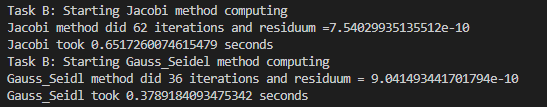
\includegraphics{zadanieB_1}\\
Algorytm Jacobiego wykonał zadanie w \textbf{62 iteracji}, które zajęły ok. \textbf{0.65s}, a zmiana normy wektora residuum w zależności od 
iteracji prezentuje się następująco.\\
Z kolei algorytm Gaussa-Seidla wykonał zadanie w \textbf{36 iteracji}, które zajęły ok.\textbf{0,37s}, a zmiana normy wektora residuum w zależności od iteracji dla 
tej metody wygląda następująco.\\
\includegraphics[scale=0.8]{zadanieB_2}\\
Jak widać metoda Gaussa-Seidla wykonuje się około 2 razy szybciej, co prawdopodobnie wynika z tego, że do obliczania kolejnych rozwiązań korzystamy nie tylko z rozwiązania w poprzedniej iteracji, ale także z aktualnie wykonwyanej iteracji.\\

\subsection{Zadanie C}
W programie zostało zaimplementowane założenie, że w przypadku metod iteracyjnych dojście do progu 1000 iteracji powinno zakończyć wywoływanie tejże metody. Na dodatek w momencie osiągnięcia normy wektora residuum rzędu \textbf{inf} powoduje także wyjście z metody.\\
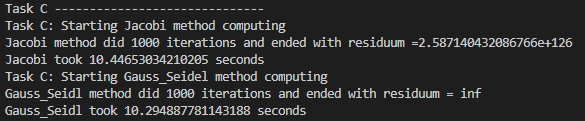
\includegraphics{zadanieC_1}\\
\includegraphics[scale=0.8]{zadanieC_2}\\
W przypadku macierzy, której wartości na głównej diagonali wynoszą 3, oba algorytmy zawiodły zwracając w/w wartości.\\
Jak wiadomo zarówno metoda Gaussa-Seidla oraz Jacobiego są metodami zwracającymi sukces przy pewnych założeniach co do macierzy \textbf{A}.
Problem związany z nierozwiązaniem układów równań z zadania C jest spowodowany zmianą wartości elementów na głównej diagonali tejże macierzy. Wydaje mi się, 
że niepowodzenie zaimplementowanych metod iteracyjnych jest stricte związane z faktem, że macierz \textbf{A} z podpunktu C nie jest diagonalnie dominująca, 
a przynajmniej jest mniej dominująca niż ta z podpunktu B.

\subsection{Zadanie D}
Algorytm LU nie jest algorytmem iteracyjnym. Jest to metoda faktoryzacji macierzy \textbf{A} na macierze L oraz U, a następnie rozwiązania dwóch układów równań 
za pomocą podstawiania wprzód oraz wstecz. W taki też sposób metoda LU została zaimplementowana.\\
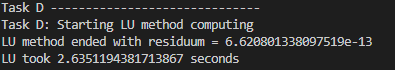
\includegraphics{zadanieD_1}\\
Dla układu równań liniowych z podpunktu C(dla którego metody iteracyjne nie działały) norma residuum rozwiązania  jest rzędu $10^{-13}$.
Czas wykonania metody LU dla tak dobrego wyniku wynosi ok. \textbf{2.63s}, co jest o wiele większym wymiarem czasowym w porównaniu do metod iteracyjnych.

\subsection{Zadanie E}
Porównanie użyteczności trzech metod rozwiązywania układów równań liniowych wymaga sprawdzenia ich czasu wykonywania względem pewnej wielkości
danych. Zakładamy także, że metody iteracyjne rozwiążą układ poprawnie, tj. norma wektora residuum będzie mniejsza niż $10^{-9}$.
W tym celu został przygotwany zbiór testowy macierzy z podpunktu A o rozmiarach $N = [500, 1000, 1500, ... , 4000]$\\
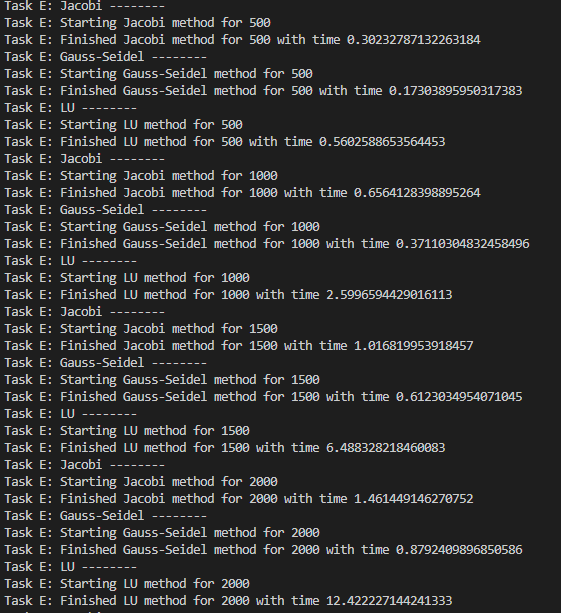
\includegraphics{zadanieE_1}
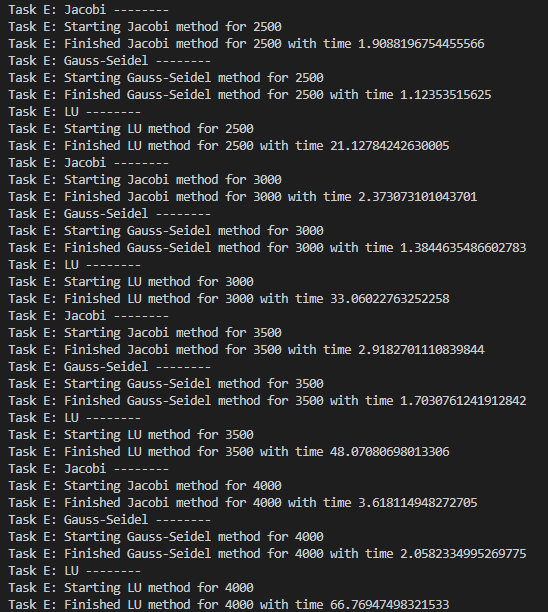
\includegraphics{zadanieE_2}
\includegraphics[scale=0.8]{zadanieE_3}\\
Widzimy, zę metody iteracyjne dla wysokich wielkości macierzy są bardzo opłacalne, ponieważ dają wyniki zadowalające w czasie niebotycznie mniejszym niż metoda LU. Z kolei przy niewielkich wartościach $N$ warto zastanowić się nad priorytetem obliczeń. Mianowicie metody iteracjyne nie oddają tak dokładnych wyników jak metoda LU, a czas jaki potencjalnie musimy dołożyc, aby rozwiązać układ równań tą metodą jest stosunkowo niewielki. Zatem czasami bardziej opłaca się zastosować metodę nieiteracyjną, aczkolwiek im większe dane posiadamy, tym bardziej opłaca się skorzystać z metody Jacobiego czy też Gaussa-Seidla. Warto także dodać że wielkim plusem metody LU jest to, że niezależnie od właściwości macierzy \textbf{A} wynik uzyskany za jej pomocą będzie na pewno prawidłowy z dosyć dużą dokładnością.\\
\end{document}